\section{Les CNNs}

\fancyhead[R]{\textit{\nouppercase{\leftmark}}}

\subsection{Le modèle du CNN}

Bien qu'étant un modèle efficace, le perceptron reste cependant coûteux en calcul : il faut réaliser les opérations matricielles sur tous les neurones de chaque couches.
Cela peut sembler exagéré, surtout dans le cas de la classification d'images. 
En effet, chercher à reconnaître des motifs sur l'image complète s'avère inutile, quand on considère qu'un motif sera localisé sur l'image, et ne sera pas dépendant des points éloignés de l'image.

C'est de cette réflexion que sont apparus les CNNs (Convolutionnal Neural Networks), qui sont entrainés à chercher des motifs sur une partie restreinte de l'image.
Le principe est le même que celui des perceptrons, sauf qu'au lieu d'appliquer un réseau entièrement connectés sur toutes les couches, on va réaliser une convolution par un "filtre" sur l'image afin de permettre la localisation de motifs.
Une couche d'un CNN est typiquement constituée de 3 éléments : 

1) Une couche de convolution

2) Une couche d'activation 

3) Une couche de pooling


La couche de convolution prend en entrée une "image" de dimension (H, L, N), H la hauteur de l'image, L sa largeur et N le nombre de channels (pour une image RGB, on a N = 3). 
Elle va ensuite lui appliquer M filtres de dimension (h', l', N) :

\begin{figure}[h]
 \centering
 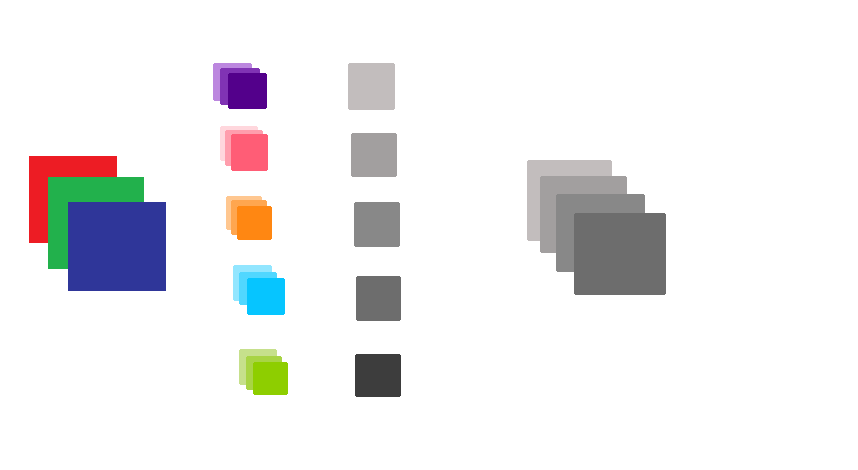
\includegraphics[width=0.7\textwidth]{img/CNN_filtres.png}
 \caption{Principe des filtres de convolution}
\end{figure}

Pour une image I de dimension (H, L, N) et un filtre F de dimension (h', l', N), on obtient une image J de dimension (H-h', L-l'), la convolution est réalisée de la manière suivante :

\begin{equation}
    J(x, y) = I \star H (x, y) = \sum_{i=0}^{h' - 1} \sum_{j=0}^{l'- 1} \sum_{n=0}^{N - 1} I(x+i, y+j, n) \times H(i, j, n)
\end{equation}

On obtient alors une sortie de dimension (H-h', L-l', M).

Intuitivement, cette partie sert à chercher la ressemblance entre le filtre et l'image : 
On devrait avoir J(x,y) < 0 si la partie de l'image I en (x,y) est très différente du filtre appliqué, et J(x,y) > 0 sinon, avec un "score" plus ou moins élevé selon la ressemblance.


On applique ensuite la couche d'activation : on utilise une fonction non-linéaire comme dans le cas du perceptron. 
Communément, la fonction utilisée pour les couches de convolution intermédiaires est la fonction reLU :

\begin{equation}
    reLU (x) = x
\end{equation} si x > 0
\begin{equation}
    reLU (x) = 0 
\end{equation} sinon


\newpage 

Cette partie sert à ramener le résultat dans les réels positifs pour éviter une divergence au niveau des calculs, et pour augmenter l'écart relatif entre un bon score et un mauvais score : un score de 0 et en score de -1 obtenu lors de la convolution sont alors considéré comme tout aussi mauvais.

Enfin, on applique une couche de pooling, qui sert à réduire le nombre de données obtenues en sortie des 2 couches précédentes.
Le pooling cherche à "résumer" les scores d'une partie de l'image, en donnant un score qui dépend des pixels de cette partie.
Il existe plusieurs méthode de pooling, comme par exemple le pooling par moyenne, ou le pooling par maximum, qui est plus utilisé en pratique :
pour une image J, on choisi un paramètre S (S < L, H), et on otient la sortie K telle que :

\begin{equation}
    K(x, y) = max_{i,j \in [0, S-1] ^2 } { J(x \times S + i , y \times S + j ) }
\end{equation}


On peut ainsi enchainer les couches de convolution jusqu'à une couche finale, qui sera ensuite reliée à un réseau complètement connecté (qui n'est rien d'autre qu'un simple perceptron), pour pouvoir exploiter les résultats obtenus jusque là.
Les poids à optimiser sont alors les poids des matrices "filtres", et les poids de la couche entièrement connectée.
Dans le principe, un CNN est comme un perceptron (à part pour la couche de pooling, on pourrait construire un CNN avec un perceptron), à l'exception que certains poids sont liés lors de l'apprentissage. 

\subsection{Application pratique}

Afin de mieux comprendre le principe du CNN, nous avons réalisé un exemple simple mais clair : 
\begin{figure}[h]
 \centering
 \includegraphics[width=0.7\textwidth]{img/cnn_exemple/}
 \caption{Image à reconnaître}
\end{figure}